% This is the ADASS_template.tex LaTeX file, 26th August 2016.
% It is based on the ASP general author template file, but modified to reflect the specific
% requirements of the ADASS proceedings.
% Copyright 2014, Astronomical Society of the Pacific Conference Series
% Revision:  14 August 2014

% To compile, at the command line positioned at this folder, type:
% latex ADASS_template
% latex ADASS_template
% dvipdfm ADASS_template
% This will create a file called aspauthor.pdf.}

\documentclass[11pt,twoside]{article}

% Do NOT use ANY packages other than asp2014. 
\usepackage{asp2014}

\aspSuppressVolSlug
\resetcounters

% References must all use BibTeX entries in a .bibfile.
% References must be cited in the text using \citet{} or \citep{}.
% Do not use \cite{}.
% See ManuscriptInstructions.pdf for more details
\bibliographystyle{asp2014}

% The ``markboth'' line sets up the running heads for the paper.
% 1 author: "Surname"
% 2 authors: "Surname1 and Surname2"
% 3 authors: "Surname1, Surname2, and Surname3"
% >3 authors: "Surname1 et al."
% Replace ``Short Title'' with the actual paper title, shortened if necessary.
% Use mixed case type for the shortened title
% Ensure shortened title does not cause an overfull hbox LaTeX error
% See ASPmanual2010.pdf 2.1.4  and ManuscriptInstructions.pdf for more details
\markboth{Diaz et al}{Docker - based Implementation for an Astronomical Data Analysis Cloud Service}

\begin{document}

\title{Docker - based Implementation for an Astronomical Data Analysis Cloud Service}

% Note the position of the comma between the author name and the 
% affiliation number.
% Author names should be separated by commas.
% The final author should be preceded by "and".
% Affiliations should not be repeated across multiple \affil commands. If several
% authors share an affiliation this should be in a single \affil which can then
% be referenced for several author names.
% See ManuscriptInstructions.pdf and ASPmanual2010.pdf 3.1.4 for more details\author{M. A. Diaz$^1$, C. Valenzuela$^1$
\author{M. Diaz$^1$, M. Araya$^1$, C. Jauregui, C. Valenzuela$^1$, L. Pizarro $^1$, M. Osorio$^1$, and M. Solar$^1$ \affil{$^1$Universidad T\'ecnica Federico Santa Mar\'ia, Valpara\'iso, Chile; \email{madiaz@alumnos.inf.utfsm.cl}} %\email{camilo.valenzuela@alumnos.usm.cl} \email{leonardo.pizarro@usm.cl} \email{mosorio@inf.utfsm.cl}
}

% This section is for ADS Processing.  There must be one line per author.
\paperauthor{M.Diaz}{madiaz@alumnos.inf.utfsm.cl}{}{Universidad Tecnica Federico Santa Maria}{Electronic Department}{Valparaiso}{V Region}{2340000}{Chile}
\paperauthor{C. Valenzuela}{camilo.valenzuela@alumnos.usm.cl}{}{Universidad Tecnica Federico Santa Maria}{Informatics Department}{Valparaiso}{V Region}{2340000}{Chile}
\paperauthor{L. Pizarro}{leonardo.pizarro@usm.cl}{0000-0003-0576-925X}{Universidad Tecnica Federico Santa Maria}{Informatics Department}{Valparaiso}{V Region}{2340000}{Chile}
\paperauthor{M. Osorio}{mosorio@inf.utfsm.cl}{}{Universidad Tecnica Federico Santa Maria}{Informatics Department}{Valparaiso}{V Region}{2340000}{Chile}
\paperauthor{M. Araya}{maray@inf.utfsm.cl}{0000-0003-3472-4130}{Universidad Tecnica Federico Santa Maria}{Informatics Department}{Valparaiso}{V Region}{2340000}{Chile}
\paperauthor{C. jauregui}{cjauregu@alumnos.inf.utfsm.cl}{}{Universidad Tecnica Federico Santa Maria}{Informatics Department}{Valparaiso}{V Region}{2340000}{Chile}
\paperauthor{M. Solar}{msolar@inf.utfsm.cl}{}{Universidad Tecnica Federico Santa Maria}{Informatics Department}{Valparaiso}{V Region}{2340000}{Chile}

\begin{abstract}
The data deluge problem that astronomy research confronts not only require developing new algorithms and computing infrastructure, but also fostering modern software and services.
% sug: The problem of the data deluge that astronomy research currently faces, besides requiring the development of new algorithms and computing infrastructure also requires the fostering of modern software and services
% before: In this context, the Cloud computing paradigm allows moving processing to where the data is, minimizing data transfer to the user and taking advantage of high-performance computing infrastructure at the datacenters.
For that matter, the cloud computing paradigm allows to perform the processing of the data where it is, minimizing the transfer to the end-user and taking advantage of the high-performance computing infrastructure of the datacenters.
% before: However, new challenges arise when these services are deployed under a high-availability principle in order to be competitive with the convenience and simplicity of local processing.
However, new challenges arise when these services are deployed under the high-availability principle in order to compete with the convenience of local processing.
Between them we found multi-user support, load balancing, resource usage optimization, securing data and network security.
% sug: Between them we found: multi-user support, load balancing, resource usage optimization, securing data and network security.
In this paper we report the architecture and caveats of the deployment of JOVIAL: a notebook-based cloud service specifically designed for astronomy using the JupyterHub platform.
% sug: ((Ok))
% before: One of the main risks of this platform is indeed its main advantage: it allows users to run arbitrary code. 
This platform allows users to run arbitrary code, which is is at the same time its main advantage and menace.
% before: We have used Docker containers to spawn a Jupyter server for each user on demand. This provides a two-fold security protection, because the user data is better protected and the host servers are better protected from the users.
Therefore, we used Docker containers to spawn a Jupyter server on demand for each user, which increased both the protection of the user data and the protection of the hosts from users.
%before: Under the high-availability principle, these dockers containers must be orchestrated to profit of the high-performance infrastructure. 
Following the high-availability principle, the containers have to be orchestrated making good use of the high-performance infrastructure.
For achieving this, we combined our user-based docker containers with the Kubernetes system, providing on-demand growth and load balancing between the hosts.
We are currently exploring supporting high-availability of the storage system through LustreFS, and managing the whole infrastructure with Rancher, a software that provides user-friendly orchestration of docker within a Kubernetes deployment.
% sug: In order to archieve this, we used the Kubernetes system on top of our user-based containers, ensuring on-demand growth and load balance between the hosts. To support high-availability we used LustreFS. We also explored the user-friendly orchestration of docker containers within a Kubernetes environment provided by Rancher to manage the whole infrastructure, ((but ended up using Kubeadm due to its higher simplicity ((and something else?)))).
% ((Not sure if "environment" is better than "deployment"))
\end{abstract}

\section{Introduction} 
%before: In a virtual observatory context, there are many challenges in the observation of a large amount of data, especially in the statistical field in order to extract knowledge from them \citep{djorgovski2003challenges}.
The Virtual Observatory (VO) is not only about data access, search and transport. The management of large volumes of data poses new challenges for data analysis, which are forcing these computations to be made at data centers rather that at personal computers. \citep{djorgovski2003challenges}.
% before: For that, there are libraries and computational tools designed to visualize and describe phenomena in those data set.
Even though specialized libraries and computational tools designed to cope with this data deluge are now available, the platforms and services to run them at high-performance environments are less developed.
%In Chilean Virtual Observatory \citep{solar2015chilean} we are building a service that helps in this task by giving a web platform to the astronomers where they can run code, export and import files in an account inside the datacenter where the virtual observatory exist.
% sug: 
In the Chilean Virtual Observatory \citep{solar2015chilean} we are building a service that provides a web platform for astronomers to run code, visualize data and export/import their files to an account at our data center.
%BEFORE: We call this platform \emph{Jovial} and includes many software and hardware coordination in its implementation. It is based on a JupyterHub server \citep{jupyter2016github} with a Kubernetes that orchestrate Docker containers \citep{bernstein2014containers}.
The implementation of this platform, that we named ``Jovial'', requires the coordination of many software and hardware components. It's based on a JupyterHub server \citep{jupyter2016github} whose Docker containers are orchestrated by Kubernetes \citep{bernstein2014containers}.
%before: Besides the users needs an account where they can save their data and codes. These files are managed by a file system called LustreFS that lets us manage a huge amount of data with low latency \citep{braam2002lustre}.
Besides this, users need an account where to save their code and data. these files are managed by the LustreFS file system that allow us to manage huge amount of data with low latency \citep{braam2002lustre}.
%All this architecture and the networking involved will be explained in the next sections.
The sections 2 explains the gradual implementation of Jovial and the section 3 explains the user experience on it.
% ((after that you do something else don't you?))

\section{Jovial}
\subsection{Jupyter Notebook and JupyterHub}

We selected Jupyter Notebook, which brings tools for programing, visualization, storage of files and other features, as our data analysis application. Each notebook in the application uses a kernel where the codes are processed, for this reason we use the Ipython kernel that allows the users to run code wrote in python.

The Jupyter Notebook server only allows one user per instance, so we implemented JupyterHub which allows multiple users, providing each user a Jupyter notebook through an account.  A user can download a dataset inside its notebook and process it using the processing power, bandwidth and disk space of the data center instead of on its own computer, additionally all the work is stored in the account. We refer at the process of bringing a notebook to a user as "spawn", and where it spawns is determined by the "spawner". 

By default the user of the account is a generic system user and the notebook spawns in the host server. This combined with the feature of running random code in the notebooks represents a risk for the server and the others users, for this reason we made two decisions:

\begin{itemize}
\item The notebooks have to spawn on an isolated instance with a limit of resources in order to keep the server and the other users safe.
\item Each user has a private account with a file system where they can store their work.
\end{itemize}
These two decisions complement each other since the notebook use the file system of the user to exist, for this, the file system must be accessible by the spawner, and the spawner has to have writing and reading permission on the files.

\subsection{Isolation and file system}
The isolation goal can be accomplished by using Docker containers, these containers recreate a system environment (like a virtual machine but lighter) inside the server, so if we spawn the notebook inside a docker container the user will only see the system of the container. To use this approach, we have to provide the container with the files of the user through a docker volume, mounting the user's file system on the host that holds the container. 

We use LustreFS to manage the users' files. LustreFS is a distributed file system optimized to operate with low latency over a large amount of data (Terabytes and Petabytes). This feature is fundamental since we work with astronomical data. The file system of the users is mounted through InfiniBand (a high performance low-level data transfer protocol) on the same server where docker containers are hosted. Then these files are passed to the containers as docker volumes.

\subsection{Cloud control}

Docker needs a host where to put its containers. This host is a node of a cluster. A node is a physical server that is a Lustre client, so it can mount the users' files. But if the node fails all the infrastructure fails. In order to make the infrastructure robust against failure of the node, we distributed the infrastructure through several nodes, so if one of these nodes fails the others can still support Jovial. 

When we talk about distributing the infrastructure we mean to spawn the notebooks in several docker containers through different nodes. These containers have to connect with the Hub. This is not a trivial task so we leave it up to Kubernetes, a Docker container orchestrator. Kubernetes decides then where to create the container based on the current load of the nodes.  If one node fails, Kubernetes will migrate all the containers to other available nodes. So Kubernetes is not only a load balancer but it ensures high availability of the infrastructure. For this reason, not only the notebooks are put in container managed by Kubernetes but also the JupyterHub server itself is put in a container (in this paper Kubernetes pods and Docker containers are treated as the same). The whole database and all the roles and daemons of Kubernetes are distributed and replicated through the nodes so that the infrastructure becomes resistant to the failure of multiple nodes.

For networking, Kubernetes uses a service called Flanneld that gives each container an IP address in a logic private network (different from the one of the nodes) that connects the containers all across the nodes \citep{zismer2016performance}. 

The implementation of Kubernetes was made by Kubeadm since the management of all the Kubernetes deployment is a complex task for a person.

\subsection{Kubernetes and the spawner}

Users are managed globally using LDAP, a software protocol that makes entries in which important data of the user is stored (the user's id, name, etc). The spawner that allows us to use Kubernetes for JupyterHub is KubeSpawner. KubeSpawner takes the id and the name of the user from LDAP, recreates the same user in the container and mounts the user's file system in the container as a docker volume. This recreated user owns the file mounted in the container since it has the same id and name as the real one. Finally, KubeSpawner runs the notebook inside the file system of the user (that is, inside the container).

\section{The Whole Picture}
% sug: ((The section name seems unrelated with its content))

\begin{figure}[ht!]
\begin{center}
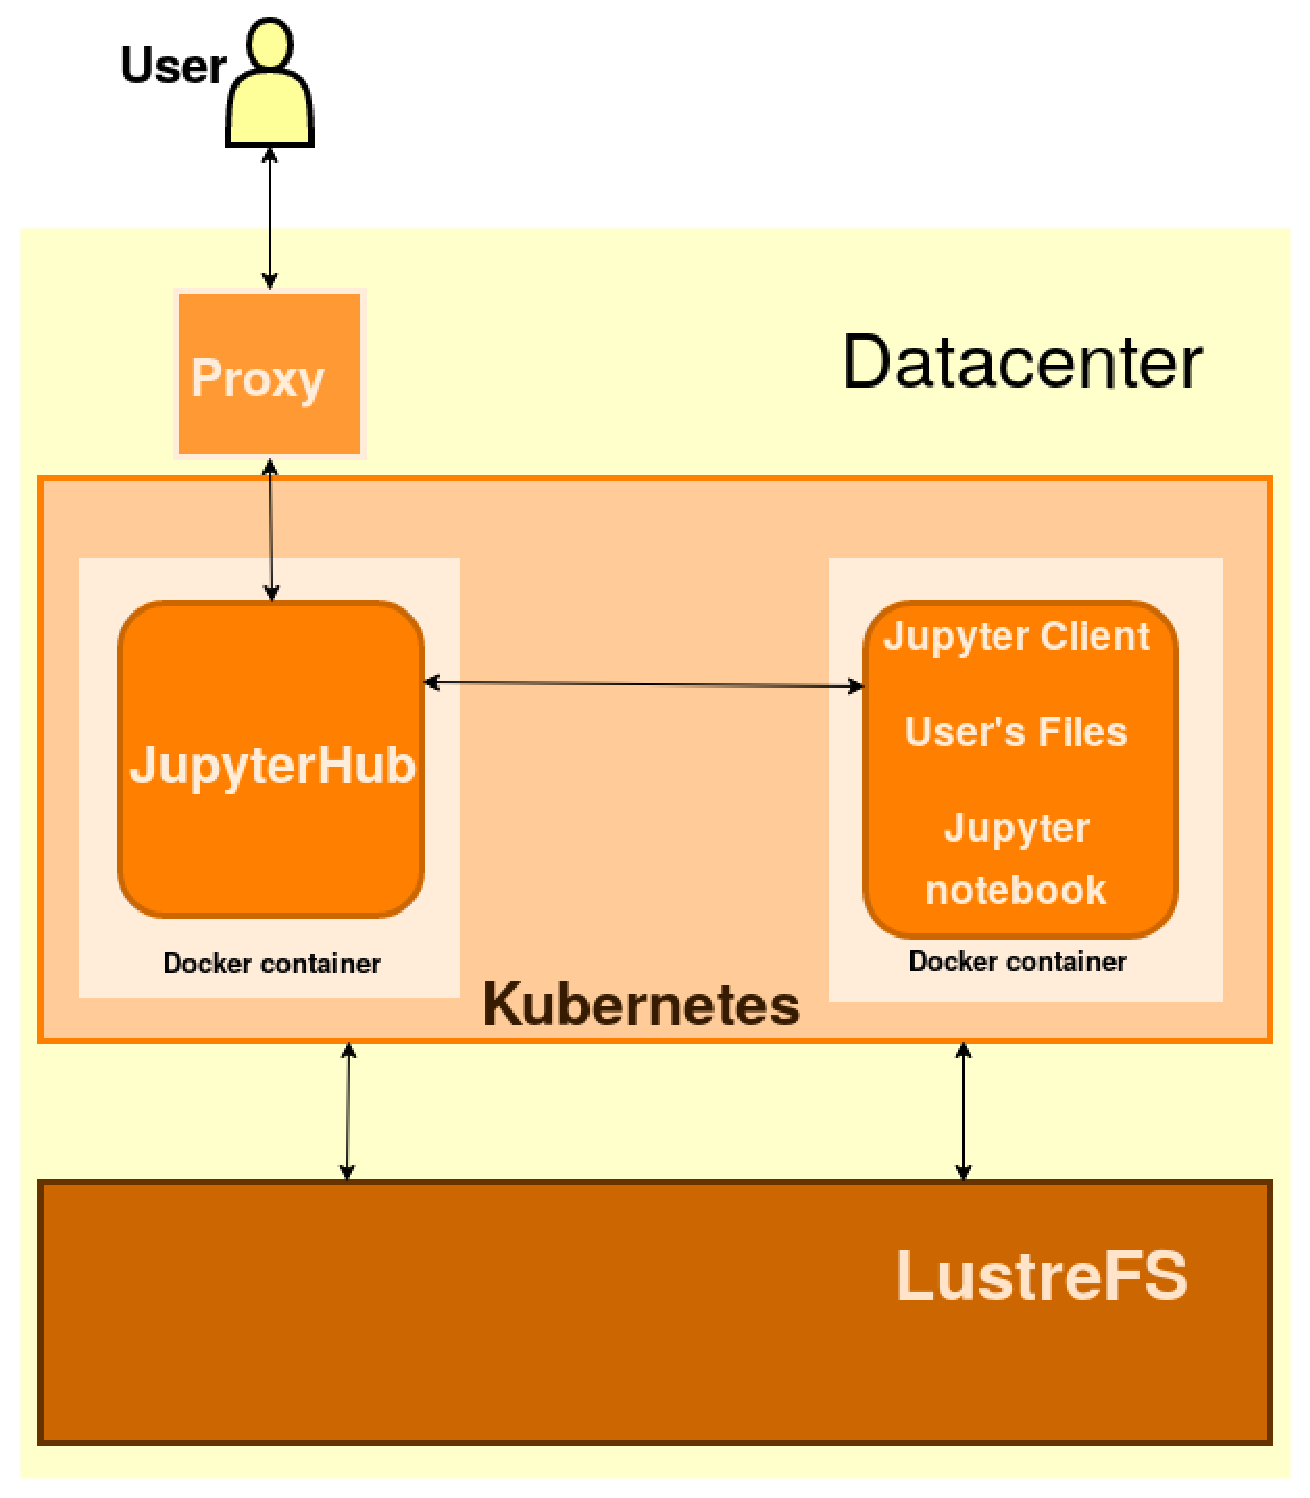
\includegraphics[width=0.6\textwidth]{P6-67_f1.eps}
\caption{Abstraction of the infrastructure.}
\label{all}
\end{center}
\end{figure}

%In general, the user enters the application through the proxy, logs in the account, and immediately the JupyterHub server looks if the container with the notebook of the user already exist. 
We keep all the servers in a private network and the public access to the JupyterHub server is gave by a proxy.

In general, the user enters the portal through the proxy and logs in with its account. Immediately, the JupyterHub server checks if the container with the Jupyter instance of the user already exists. If not, it asks Kubernetes to create it, spawns the files of the user into the container and contacts the server. An overview of the components that participate in this process is shown in Figure~\ref{all}.

% * <maxiosorio@gmail.com> 2017-10-12T14:18:32.436Z:
% Can you talk about containers?: Containers are secure and your data is secure in the containers 
% 
% ^.


\section{Conclusion}

%The objective of Jovial is that users can log in with an account to a web application, upload or download files, and download to their account astronomical data from the virtual observatory with the speed of the local network, process this data with the power of the physical server and save the result in their files or whatever storage they want. 
The objective of Jovial is to allow users to login to a personal account at a web application, download astronomical data from the virtual observatory to this account at the speed of the local network, and upload and download files selectively to their computers or another storage media.
%(("whatever" sounds a little aggressive, btw)) ((Also, should you mention again the possibility of uploading code through a Jupiter notebook and process the datasets with the resources of the datacenter?))

%With the notebooks inside containers and distributed we can control the correct use of ours resources and prevent users to compromises the server or other users experience.
With the notebooks distributed and confined to containers we can control the correct use of ours resources and prevent the users to compromise the server or the work of other users. 
%The implementation of these tools in particular was thought in order to ensure high availability of the service and the protection of users' data. 
The selection and arrangement of these particular tools was done in order to ensure high availability of the service and the protection of users' data. 

\acknowledgments This work has been partially funded by - FONDEF IT 15I10041. An special thanks to the JupyterHub team for their support on this project.
\bibliography{P6-67}  % For BibTex


\end{document}



brainstorm


